\section{Metoda Eulera pierwszego rzędu}
%%%%%%%%%%%%%%%%%%%%%%%%%%
\begin{frame}{Metoda Eulera pierwszego rzędu}
  \underline{$f(u,t)$= ?} \quad dla  \quad $t \in [t^n,t^{n+1}] \approx f(u^n,t^n)$
  \begin{figure}
	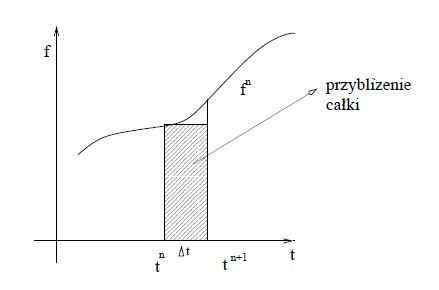
\includegraphics[height=0.65\textheight]{img/22/img1.jpg}
	\end{figure}
\end{frame}
%%%%%%%%%%%%%%%%%%%%%%%%%%
\begin{frame}{Cechy metody}
  \textbf{Algorytm:}
  $$u^{n+1} = u^n - f(u^n, t^n) \cdot \Delta t$$
  \textbf{Cechy:}
  \begin{itemize}
    \item jawna
    \item dokładna jedynie do wyrazów 1-go rzędu ze względu na $\Delta t$ \quad $(\varepsilon=0(\Delta t)$)
    \item prosta
    \item efektywna
  \end{itemize}
\end{frame}
%%%%%%%%%%%%%%%%%%%%%%%%%%
\begin{frame}{Stabilność}
  $t^n$ \quad $u^n, \varepsilon^n$ - błąd \qquad
  $t^{n+1}$ \quad $u^{n+1}, \varepsilon^{n+1}$ 
  \fbox{$\varepsilon^{n+1} = g \cdot \varepsilon^n$\qquad
  g - współczynnik wzmocnienia błędu}

  $$u^{n+1} + \varepsilon^{n+1} = u^n+\varepsilon^n-f(u^n+\varepsilon^n,t^n)\cdot \Delta t \qquad(*)$$
  \underline{zał.:} $\varepsilon^n$ - mały $\Rightarrow$ linearyzacja r. nieliniowego
  $$f(u^n+\varepsilon^n,t^n) = f(u^n,t^n)+\frac{\partial f}{\partial u}{\bigg\arrowvert}_{u^n} \cdot \varepsilon^n+0(\varepsilon^n)$$
  Po podst. do (*):\qquad $\varepsilon^{n+1} = \varepsilon^n-\frac{\partial f}{\partial u}\big\arrowvert_n \cdot \Delta t \cdot \varepsilon^n +0(\varepsilon^n)$ \newline
  \underline{współczynnik wzmocnienia}:\qquad $g = 1- \frac{\partial f}{\partial u}{\big\arrowvert}_n \cdot \Delta t\downarrow$
  warunek stabilności: $|g|<1$ warunek stabilności dla $\frac{\partial f}{\partial u}>0$
  $$\frac{\partial f}{\partial u}\arrowvert_n \cdot \Delta t \leqslant 2 \quad 
  \rightarrow \quad \Delta t \leqslant \frac{2}{\frac{\partial f}{\partial u}\arrowvert_n} \Rightarrow krok$$
  (gdy $\frac{\partial f}{\partial u}\arrowvert_n < 0$ - metoda niestabilna)
\end{frame}
%%%%%%%%%%%%%%%%%%%%%%%%%%

\begin{frame}{Przykład}
	\begin{center}
	$\frac{du}{dt}+\frac{u}{\tau} = 0$, \quad $u(0) = 1$\newline $R$, $L\rightarrow \tau = \frac{L}{R}$\qquad rozpad promieniotwórczy\par
      \begin{itemize}
    \item analitycznie: $u = e^{-\frac{t}{\tau}}$
    \end{itemize}
	\end{center}
  
  krok czasowy gwarantujący stabilność:
  $$\frac{\partial f}{\partial u}\bigg\arrowvert_n = \frac{1}{\tau}\qquad \Delta t \leqslant 2\tau$$
  $\Rightarrow$ \underline{stabilność} - fundamentalna własność metody różnicowej
\end{frame}
%%%%%%%%%%%%%%%%%%%%%%%%%%

\begin{frame}{Przykład 2 - równanie typu oscylacyjnego}
	\begin{center}
		oscylator harmoniczny: \qquad $\frac{d^2x}{dt^2}+ \omega^2x=0$
	\end{center}
    $\Rightarrow$ układ 2 równań:
    $$\left\{\begin{array}{lccll}
	\frac{dx}{dt}&-&\omega^2x&=&0\\
	\frac{dx}{dt}&+&\omega v&=&0\\
	\end{array} \right.$$
    wprowadzenie \qquad \underline{$u = x+iv$} $\Rightarrow$ pojedyncze równanie 1-go rzędu:
    $$ \frac{du}{dt} + i\omega u= 0 \qquad \arrowvert \qquad bo: \quad \frac{dx}{dt} + i\frac{dv}{dt}+i\omega v = 0$$
    \underline{współczynnik wzmocnienia:}
    $$g = 1-{\frac{\partial f}{\partial u}}\bigg\arrowvert _n \cdot \Delta t \quad \Rightarrow \quad g=1-i\cdot \omega \cdot \Delta t \qquad zespolony!$$
\end{frame}
%%%%%%%%%%%%%%%%%%%%%%%%%%

\begin{frame}{Przykład 2 c.d.}
	$$|g|^2 = g \cdot g^* = 1+\omega^2 {\Delta t}^2 \quad \rightarrow \quad 1+\bigg(\frac{\partial f}{\partial u}\bigg{\arrowvert}_n \cdot \Delta t\bigg)^2 > 1 \Rightarrow |g| > 1 $$
    \begin{block}{Uwaga}
    	Metoda Eulera jest bezwzględnie niestabilna dla równań typu oscylacyjnego.
    \end{block}
    W zagadnieniach \textit{nieliniowych $\frac{\partial f}{\partial u}$} jest funkcją $u$ \quad $\Rightarrow$ \quad należy na każdym etapie wybierać $\Delta t$ spełniające warunki stabilności. 
\end{frame}
%%%%%%%%%%%%%%%%%%%%%%%%%%
